\documentclass[11pt,compress,t,notes=noshow, aspectratio=169, xcolor=table, usenames,dvipsnames]{beamer}

\usepackage{../../style/lmu-lecture}
% Defines macros and environments
% This file is included in slides and exercises

% Rarely used fontstyle for R packages, used only in 
% - forests/slides-forests-benchmark.tex
% - exercises/single-exercises/methods_l_1.Rnw
% - slides/cart/attic/slides_extra_trees.Rnw
\newcommand{\pkg}[1]{{\fontseries{b}\selectfont #1}}

% Spacing helpers, used often (mostly in exercises for \dlz)
\newcommand{\lz}{\vspace{0.5cm}} % vertical space (used often in slides)
\newcommand{\dlz}{\vspace{1cm}}  % double vertical space (used often in exercises, never in slides)
\newcommand{\oneliner}[1] % Oneliner for important statements, used e.g. in iml, algods
{\begin{block}{}\begin{center}\begin{Large}#1\end{Large}\end{center}\end{block}}

% Don't know if this is used or needed, remove?
% textcolor that works in mathmode
% https://tex.stackexchange.com/a/261480
% Used e.g. in forests/slides-forests-bagging.tex
% [...] \textcolor{blue}{\tfrac{1}{M}\sum^M_{m} [...]
% \makeatletter
% \renewcommand*{\@textcolor}[3]{%
%   \protect\leavevmode
%   \begingroup
%     \color#1{#2}#3%
%   \endgroup
% }
% \makeatother


\title{Interpretable Machine Learning}
% \author{LMU}
%\institute{\href{https://compstat-lmu.github.io/lecture_iml/}{compstat-lmu.github.io/lecture\_iml}}
\date{}

\begin{document}


% Set style/preamble.Rnw as parent.

% Load all R packages and set up knitr

% This file loads R packages, configures knitr options and sets preamble.Rnw as
% parent file
% IF YOU MODIFY THIS, PLZ ALSO MODIFY setup.Rmd ACCORDINGLY...

% Defines macros and environments

 \newcommand{\titlefigure}{figure/counterfactuals_obj}
\newcommand{\learninggoals}{
\item Formulate CEs as optimization problem
\item Identify key objectives (proximity, sparsity)
\item Understand trade-offs in CE generation}

\lecturechapter{CE: Optimization Problem and Objectives}
\lecture{Interpretable Machine Learning}


\begin{frame}{Mathematical Perspective}
	Terminology:
	\begin{itemize}
		\item $\xv$: original/factual datapoint whose prediction we want to explain
		\item $y' \subset \R^g$: desired prediction ($y' =$ ``grant credit") or interval ($y' = [1000, \infty[$)
	\end{itemize}
	\lz\pause
	A \textbf{valid} counterfactual $\xv'$ satisfies two criteria:
	\begin{enumerate}
    \item \textbf{Prediction validity:} CE's prediction $\fh(\xv')$ is equal to the desired prediction $y'$ 
\item \textbf{Proximity:} CE $\xv'$ is as close as possible to the original input $\xv$
		% \item whose prediction $\fh(\xv')$ is equal to the desired prediction $y'$ (prediction validity)
		% \item maximally close to the original datapoint $\xv$ (proximity)
	\end{enumerate}
	\lz\pause
	Reformulate these two objectives as optimization problem: %(denoted by $o_1$ and $o_2$)
	
$$\argmin_{\xv'} \lambda_1 o_{target}(\fh(\xv'), y') + \lambda_2 o_{proximity}(\xv', \xv)$$

	\begin{itemize}
		\item $\lambda_1$ and $\lambda_2$ balance the two objectives
          \item $o_{target}$: distance in target space %(e.g., cross-entropy, margin loss)
          \item $o_{proximity}$: distance in feature space % (e.g., $\ell_1$, Mahalanobis, cost-aware)
		%\item Choice of $o_{target}$ (distance on target space) and of $o_{proximity}$ (distance on feature space) is crucial
	\end{itemize}
\end{frame}



\begin{frame}{Objective Functions \citebutton{Dandl et al. (2020)}{https://arxiv.org/abs/2004.11165}}

\textbf{Distance in target space $o_{target}$:}

\begin{itemize}
  \item \textbf{Regression:} L$_1$ distance   
  $o_{target}(\fh(\xv'), y') = | \fh(\xv') - y'|$
  
  \item \textbf{Classification:}  
  \begin{itemize}
    \item For predicted probabilities: $o_{target} = | \fh(\xv') - y'|$
    \item For predicted hard labels: $o_{target} = \mathbb{I} \{ \fh(\xv') \ne y'\}$
  \end{itemize}
\end{itemize}

\pause

\textbf{Distance in input space $o_{proximity}$: Gower distance (mixed feature types)}

\[
o_{proximity}(\xv', \xv) = \Gower(\xv', \xv) = \frac{1}{p} \sum_{j = 1}^{p} \delta_G(x'_j, x_j) \in [0, 1], \text{ where}
\]

% \begin{equation*}
% \delta_G(x'_j, x_j) = 
% \begin{cases}
% \frac{1}{\widehat{R}_j} \, |x'_j - x_j| & \text{if $x_j$ is numerical} \\
% \mathbb{I} \left\{ x'_j \ne x_j \right\} & \text{if $x_j$ is categorical}
% \end{cases}
% \end{equation*}

\begin{itemize}
  \item $\delta_G(x'_j, x_j) = \mathbb{I} \left\{ x'_j \ne x_j \right\}$ if $x_j$ is categorical
  \item $\delta_G(x'_j, x_j) = \frac{1}{\widehat{R}_j} \, |x'_j - x_j| $ if $x_j$ is numerical\\
  $\leadsto \widehat{R}_j$ is the range of feature $j$ in the training set to ensure $\delta_G(x'_j, x_j) \in [0, 1]$
\end{itemize}

\end{frame}


% \begin{frame}{Mathematical Perspective \citebutton{Dandl et al. (2020)}{https://arxiv.org/abs/2004.11165}}
	
% 	\begin{itemize}
% 		\item Regression: $o_{target}$ could be the L$_1$-distance $o_{target}(\fh(\xv'), y') = |\fh(\xv')-y'|$
% 		\item Classification:
% 		L$_1$-distance for scores and 0-1 Loss for labels, e.g., $o_{target}(\fh(\xv'), y') = \ind_{\{ \fh(\xv') \neq y' \}}$
% 		\pause
% 		\item $o_{proximity}$ could be the Gower distance (suitable for mixed feature space):
% 		$$o_{proximity}(\xv', \xv) = \Gower(\xv', \xv) = \frac{1}{p}\sum_{j = 1}^{p} \delta_G(x'_j, x_j)	\in [0, 1]$$
% 		The value of $\delta_G$ depends on the feature type (numerical or categorical):
% 		\begin{equation*}
% 		\delta_G(x'_j, x_j) =
% 		\begin{cases}
% 		\frac{1}{\widehat{R}_j}|x_j'- x_j| & \text{if $x_j$ is numerical} \\
% 		\ind_{\{ x_j' \neq x_j \}} & \text{if $x_j$ is categorical}
% 		\end{cases}
% 		\end{equation*}
% 		with $\widehat{R}_j$ as the value range of feature $j$ in the training dataset (to ensure that $\delta_G(x'_j, x_j)	\in [0, 1]$)
% 	\end{itemize}
% %\footnote[frame]{Dandl S., Molnar C., Binder M., Bischl B. (2020) Multi-Objective Counterfactual Explanations. In: Bäck T. et al. (eds) Parallel Problem Solving from Nature – PPSN XVI. PPSN 2020. Lecture Notes in Computer Science, vol 12269. Springer, Cham.}
% %\footnote[frame]{Verma et al. (2020). \href{https://arxiv.org/pdf/2010.10596.pdf}{Counterfactual Explanations for Machine Learning: A Review.}}
% \end{frame}

\begin{frame}{Further Objectives: Sparsity}
	%While validity is a necessary condition for counterfactuals,
	Additional constraints can improve the explanation quality of the corresponding CEs\\
	$\leadsto$ popular constraints include \textbf{sparsity} and \textbf{plausibility}
	
	\lz

	\textbf{Sparsity} Favor explanations that change few features
	\begin{itemize}[<+->]
		\item End-users often prefer short over long explanations%\\
        \item Sparsity could be integrated into $o_{proximity}$ \\
        e.g., using L$_0$-norm (number of changed features) or L$_1$-norm (LASSO)
		%$\leadsto$ %changes made to obtain
		%counterfactuals should be \textbf{sparse} %(i.e., only few feature values should change)
		%\item Objective $o_{proximity}$ can take the number of changed features into account (but does not have to)\\
		%$\leadsto$ e.g., the L$_0$- and the L$_1$-norm (similar to LASSO) can do this
%		\item There could be a trade-off between the number of features changed and the total amount of change made to obtain a certain prediction.
        \item Alternative: Include separate objective measuring sparsity, e.g., via L$_0$-norm
        %we can also account for sparsity by adding an extra term to our objective that counts the number of changed features via the L0-norm
        $$o_{sparse}(\xv', \xv) = \sum_{j = 1}^p {\ind}_{\{ x'_j \neq x_j \}}$$
	\end{itemize}
\end{frame}

\begin{frame}{Further Objectives: Plausibility}
		\textbf{Plausibility:}
		\begin{itemize}
			%\item CEs should suggest alternatives that are plausible -- e.g, it is a bad idea to suggest a loan applicant to raise her income and get unemployed at the same time
			\item<1-> CEs should suggest realistic (i.e., plausible) alternatives\\
			$\leadsto$ Implausible: increase income \emph{and} become unemployed
            %e.g., not plausible to suggest to raise your income and get unemployed at the same time
			\item<2-> CEs should adhere to data manifold or originate from distribution of $\Xspace$\\
			$\leadsto$ Avoid unrealistic combinations of feature values
			%We desire realistic CEs in the sense that they originate from the distribution of $\Xspace$ or adhere to the data manifold
			\item<3-> Estimating joint distribution is hard, especially for mixed feature spaces\\
			$\leadsto$ Common proxy: ensure that $\xv'$ is close to training data $\Xmat$
		\end{itemize}	
	\only<4>{
	\begin{columns}[c, totalwidth=\textwidth]
	\begin{column}{0.43\textwidth}
	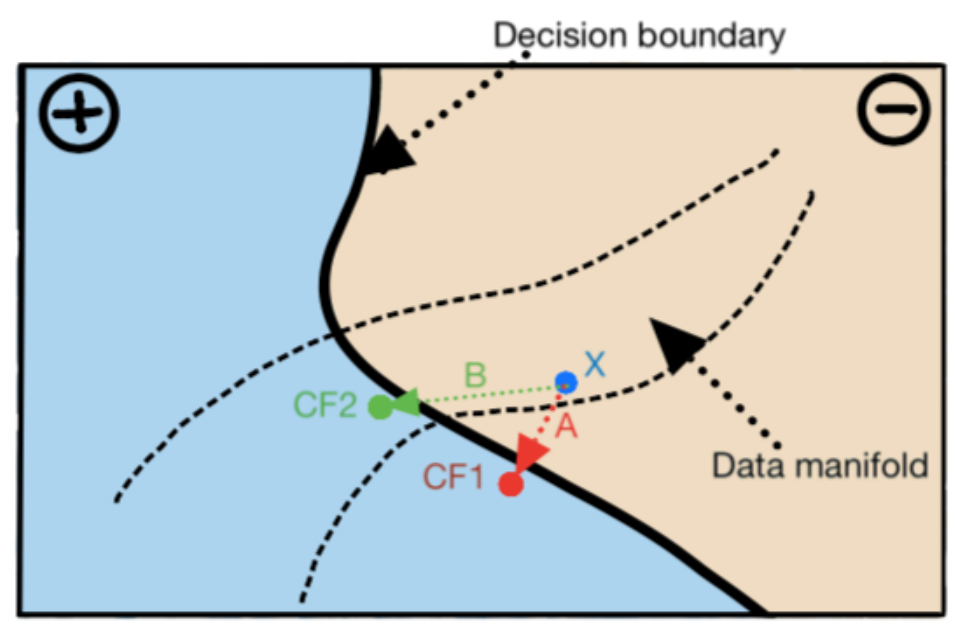
\includegraphics[width=1\textwidth]{figure/counterfactuals_obj}			
	\end{column}
	\begin{column}{0.56\textwidth}

\textbf{Example from \citebutton{Verma et al. (2020)}{https://arxiv.org/abs/2010.10596}} 
\begin{itemize}
    \item Input \textcolor{blue}{$\xv$} originally classified as $\pmb{\circleddash}$ 
    \item Two valid CEs in class $\pmb\oplus$: {\color{Red} CF1} and {\color{Green} CF2}
    \item {\color{Red} Path \textbf{A} (CF1)} is shorter (but unrealistic)
    \item {\color{Green} Path \textbf{B} (CF2)} is longer but in data manifold
\end{itemize}
%Two possible paths for \textcolor{blue}{$\xv$},			originally classified in the negative class. The two counterfactuals (\textcolor{red}{CF1} and \textcolor{green}{CF2}) are valid. Note that the red path $A$ for CF1 is the shortest, whereas the green path $B$ for CF2 adheres closely to the manifold of the training data, but is longer.
\end{column}
\end{columns}
}
%\footnote[frame]{Verma et al. (2020). \href{https://arxiv.org/pdf/2010.10596.pdf}{Counterfactual Explanations for Machine Learning: A Review.}}

\end{frame}


\begin{frame}{Further Objectives}
	%\begin{itemize}
	%\item 
%For example, $o_{plausibe}$ could then be the Gower distance of $\xv'$ to the nearest data point of the training dataset $\xv^{[1]}$

% To ensure plausibility, $o_{plausibe}$ could, e.g., be the Gower distance of $\xv'$ to its nearest data point of the training dataset which we denote $\xv^{[1]}$:
\textbf{Plausibility term:} Encourage counterfactuals close to observed data.

\begin{itemize}
  \item Define $\xv^{[1]}$ as the nearest neighbor of $\xv'$ in the training set $\Xmat$
  \item Use Gower distance between $\xv'$ and $\xv^{[1]}$ to define plausibility objective: 
$$o_{plausibe}(\xv', \Xmat) = \Gower(\xv', \xv^{[1]}) = \frac{1}{p} \sum_{j = 1}^{p}  \delta_G(x_j', x^{[1]}_j)$$
\end{itemize}


\pause

\textbf{Extended optimization:} Add sparsity and plausibility terms to the objective

\[
\argmin_{\xv'} \lambda_1 o_{\text{target}}(\fh(\xv'), y') 
+ \lambda_2 o_{\text{proximity}}(\xv', \xv)
+ \lambda_3 o_{\text{sparse}}(\xv', \xv) 
+ \lambda_4 o_{\text{plausible}}(\xv', \Xmat)
\]
%\end{itemize}

% We can extend the previous optimization problem by adding $o_{sparse}$ (for sparsity) and $o_{plausibe}$ (for plausibility):

% $$\argmin_{\xv'} \lambda_1 o_{target}(\fh(\xv'), y') + \lambda_2 o_{proximity}(\xv', \xv) + \lambda_3 o_{sparse}(\xv', \xv) + \lambda_4 o_{plausibe}(\xv', \Xmat)$$

\end{frame}


\begin{frame}{Remarks: The Rashomon Effect}
%The solution to the optimization problem might not be unique, there can be many equally close inputs that obtain the desired classification. Correspondingly, there can be many different equally good explanations for the same decision. This is called the \textbf{Rashomon effect}.

\textbf{Issue (\textbf{Rashomon effect}):}
\begin{itemize}
    \item Solution to the optimization problem might not be unique
    \item Many equally close CE might exist that obtain the desired prediction\\
    $\Rightarrow$ Many different equally good explanations for the same decision exist
\end{itemize}

\lz\pause

\textbf{Possible solutions:}
	\begin{itemize}
	\item Present all CEs for $\xv$ (but: time and human processing capacity is limited)
		%\item We could present all CEs for a given case; however, time is limited and so is the human processing capacity
		%\item Another solution is to focus on one or few CEs; however, by which criterion should they be selected?
		\item Focus on one or few CEs (but: by which criterion should guide this choice?)
	\end{itemize}
	
\lz\pause

\textbf{Note:}
	\begin{itemize}
      \item Nonlinear models can produce diverse and inconsistent CEs\\
  $\leadsto$ suggest both increasing and decreasing credit duration (confusing for users)
  \item Handling this \textbf{Rashomon effect} remains an open problem in interpretable ML
  %       \item As the model is generally non-linear, inconsistent and diverse CEs can arise\\
  %       e.g. suggesting either an increase or decrease in credit duration (confuses the explainee)
		% \item How to deal with the Rashomon effect is considered an open problem in IML
	\end{itemize}
\end{frame}

\begin{frame}{Remarks: Model or Real-World}

	\begin{itemize}
	\item CEs explain model predictions, but may appear to explain the real-world users\\
$\leadsto$ Transfer of model explanations to explain real-world is generally not permitted
  \item \textbf{Example:} CE suggests increasing age by 5 to receive a loan\\
  $\leadsto$ The applicant waits 5 years and reapplies
  \pause
  \item \textbf{Problem:} Other features may change in the meantime (e.g., job status, income)  
  %$\leadsto$ Age is causally linked to other variables\\
  $\leadsto$ \citebutton{Karimi et al. (2020)}{https://arxiv.org/abs/2002.06278} propose CEs that respect causal structure
  \item \textbf{Model drift:} Bank's algorithm itself may change over time\\
  $\leadsto$ Past CEs may become invalid
	% \item Consider a CE that proposes to increase the feature age by 5 to obtain the loan\\
	% $\leadsto$ a loan applicant takes this information and applies 5 years later for the loan
	% \item However, by then, many 
	% %of their 
	% other feature values 
	% %properties 
	% might have changed\\
	% $\leadsto$ not only age, also other causally dependent features e.g. job status might have changed \\%after 5 years% since they are causally dependent on age like income or the job status
	% $\leadsto$ \citebutton{Karimi et al. (2020)}{https://arxiv.org/abs/2002.06278} avoid this by considering causal dependencies between features
	% \item Also, the bank's algorithm might change and previous CEs are not applicable anymore
	%\item Even worse, the user might have typos in the application and in fact no changes are necessary to obtain the loan.
%		\item Actionability: We could further strengthen above's plausibility criterion by requiring counterfactuals that do not change immutable features (e.g., race, city of birth, sex). Therefore, we could  search for counterfactuals only among a defined feasible set of counterfactuals $\mathcal{A}$.
%		\item Causality: We could also restrict the search to counterfactuals that maintain any known causal relations. In the real world, if one feature is changed it affects also other features. E.g., better skills lead to better salary, but also a higher age due to the necessary training.
	\end{itemize}
%\footnote[frame]{Karimi et al. (2021). Algorithmic Recourse: From Counterfactual Explanations to Interventions.  Proceedings of the 2021 ACM Conference on Fairness, Accountability, and Transparency. 353–362.}
\end{frame}



\endlecture
\end{document}
